The following section contains the supplemental results of the effects of our missing data parameters and the different tree inference methods on the the ability to recover the "best" topology that are briefly discussed in the main body of the paper. For clarity, in the paper, we focused on the results of the effects of our missing data parameters on the Maximum Likelihood trees topology and the Bayesian consensus trees topology. The following additional results presented here give a greater insight into the effect of our missing data parameters on the Maximum Likelihood Bootstrapped trees topologies and the Bayesian posterior trees distribution topologies. Also we present here the pairwise comparisons between each parameters states for the Maximum Likelihood tree topology, the Maximum Likelihood Bootstrapped trees topologies and the Bayesian posterior trees distribution topologies.

\begin{figure} 
\centering
    \includegraphics[width=1\textwidth]{OnlineAppendices-LaTeXSuppFiles/SupplementaryFigures/Boot+Bayt-AllParam-RF+Tr-BW.pdf}
    \caption{Effect of increasing missing data on topological recovery using Maximum Likelihood Bootstrap trees (black) and Bayesian posterior tree distribution (grey). The x axis shows the percentage of missing data from 0\% (white) to 75\% (black) for the three parameters: $M_{L}$ (upper line), $M_{F}$ (middle line) and $M_{C}$ (lower line). Topological recovery was measured using two different tree comparison metrics: Normalised Robinson-Foulds distance (upper row) and Normalised Triplets distance (lower row). The graph shows the modal value (points), and the 50\% (thick solid lines) and 95\% (thin dashed lines) confidence intervals of the distributions of the tree comparison metric for each missing data parameter and tree inference method.} 
\label{Fig_Supp_BootBayt_allparam} 
\end{figure}

\begin{figure} 
\centering
     %Hide this figure for 'fast' build
%    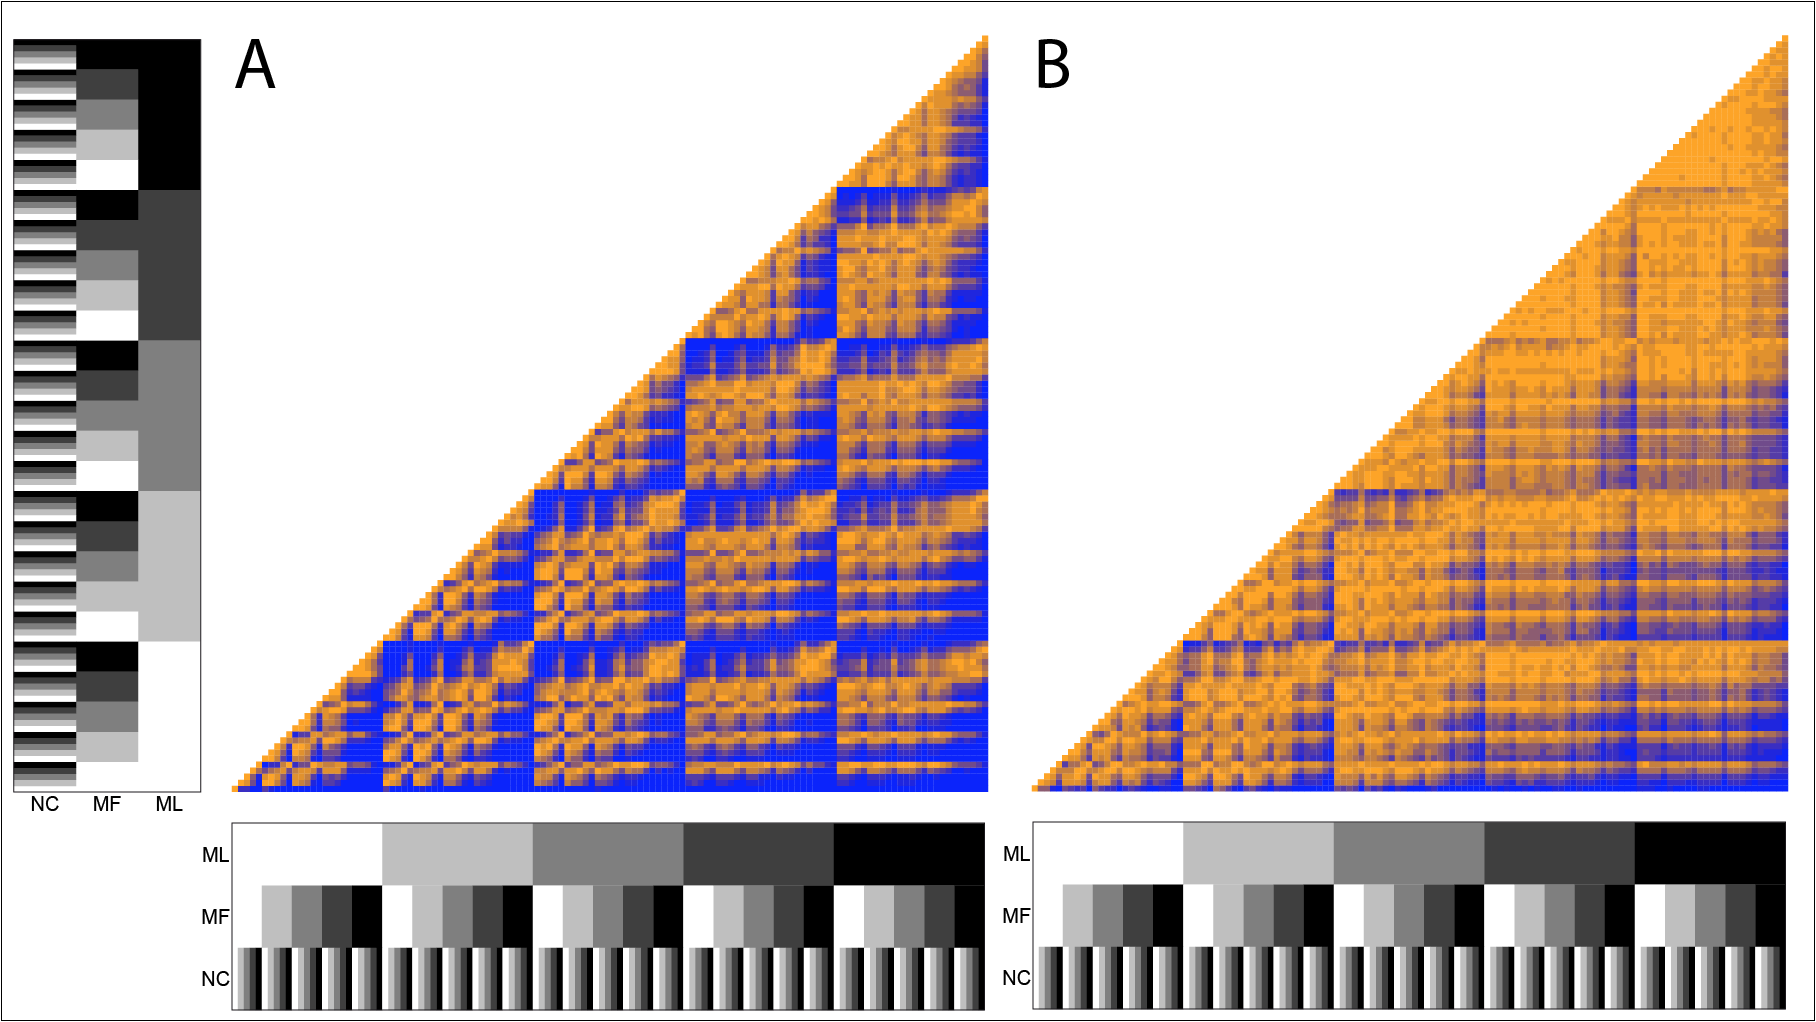
\includegraphics[width=1\textwidth]{Figures/Supplementary/PairwiseComp-ML-RF+Tr-colour.pdf}
    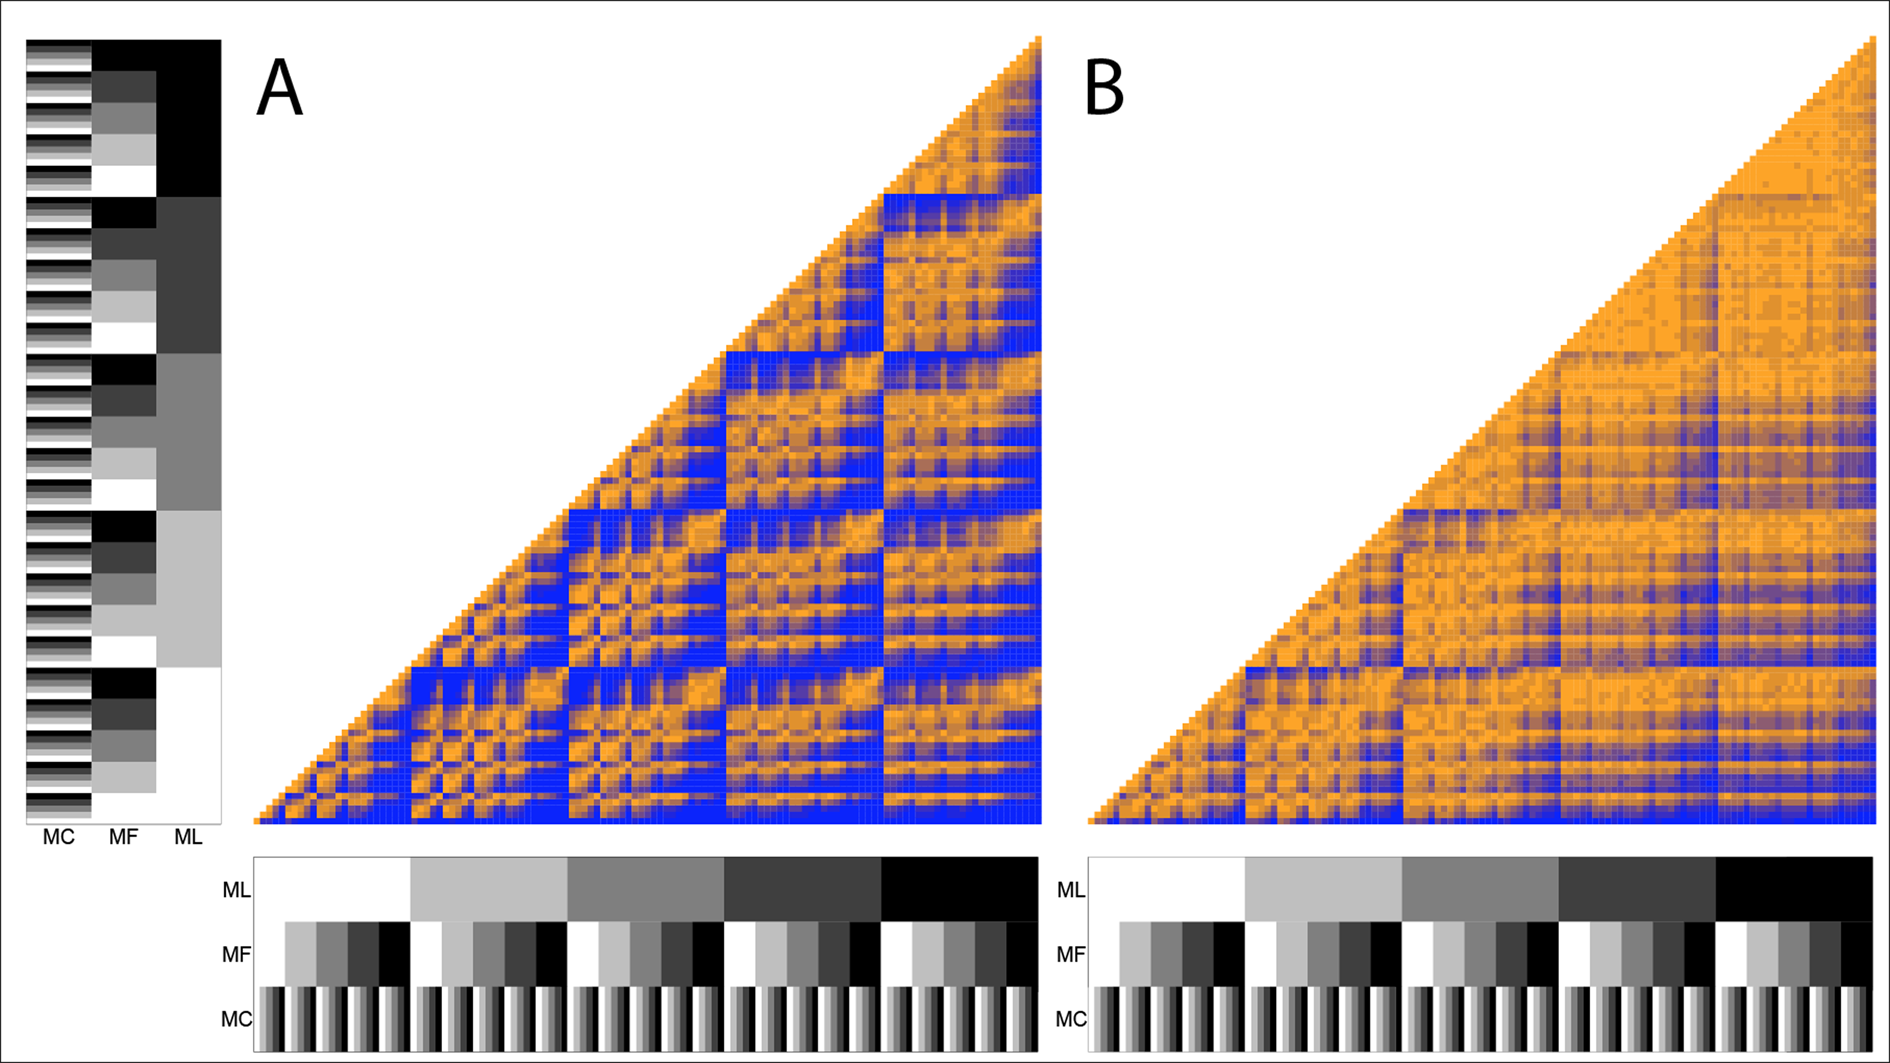
\includegraphics[width=1\textwidth]{OnlineAppendices-LaTeXSuppFiles/SupplementaryFigures/PairwiseComp-ML-RF+Tr-colour.png} %bitmap version - 300 dpi RGB
    \caption{The effects of missing data on topological recovery using Maximum Likelihood trees. The x and the y axes both show show the percentage of missing data from 0\% (white) to 75\% (black) for the three parameters: $M_{L}$ (upper line), $M_{F}$ (middle line) and $M_{C}$ (lower line). Topological recovery is represented by the probability of (A) Normalised Robinson-Foulds distance and (B) Normalised Triplets distance distributions overlapping with the "best" tree distribution, calculated using the Bhattacharyya Coefficient. The Bhattacharyya Coefficient values are indicated using a color gradient ranging from low probability of overlap in blue, to a high probability of overlap in orange.}
\label{Fig_Supp_paircomp_ML}
\end{figure} 

\begin{figure} 
\centering
     %Hide this figure for 'fast' build
%    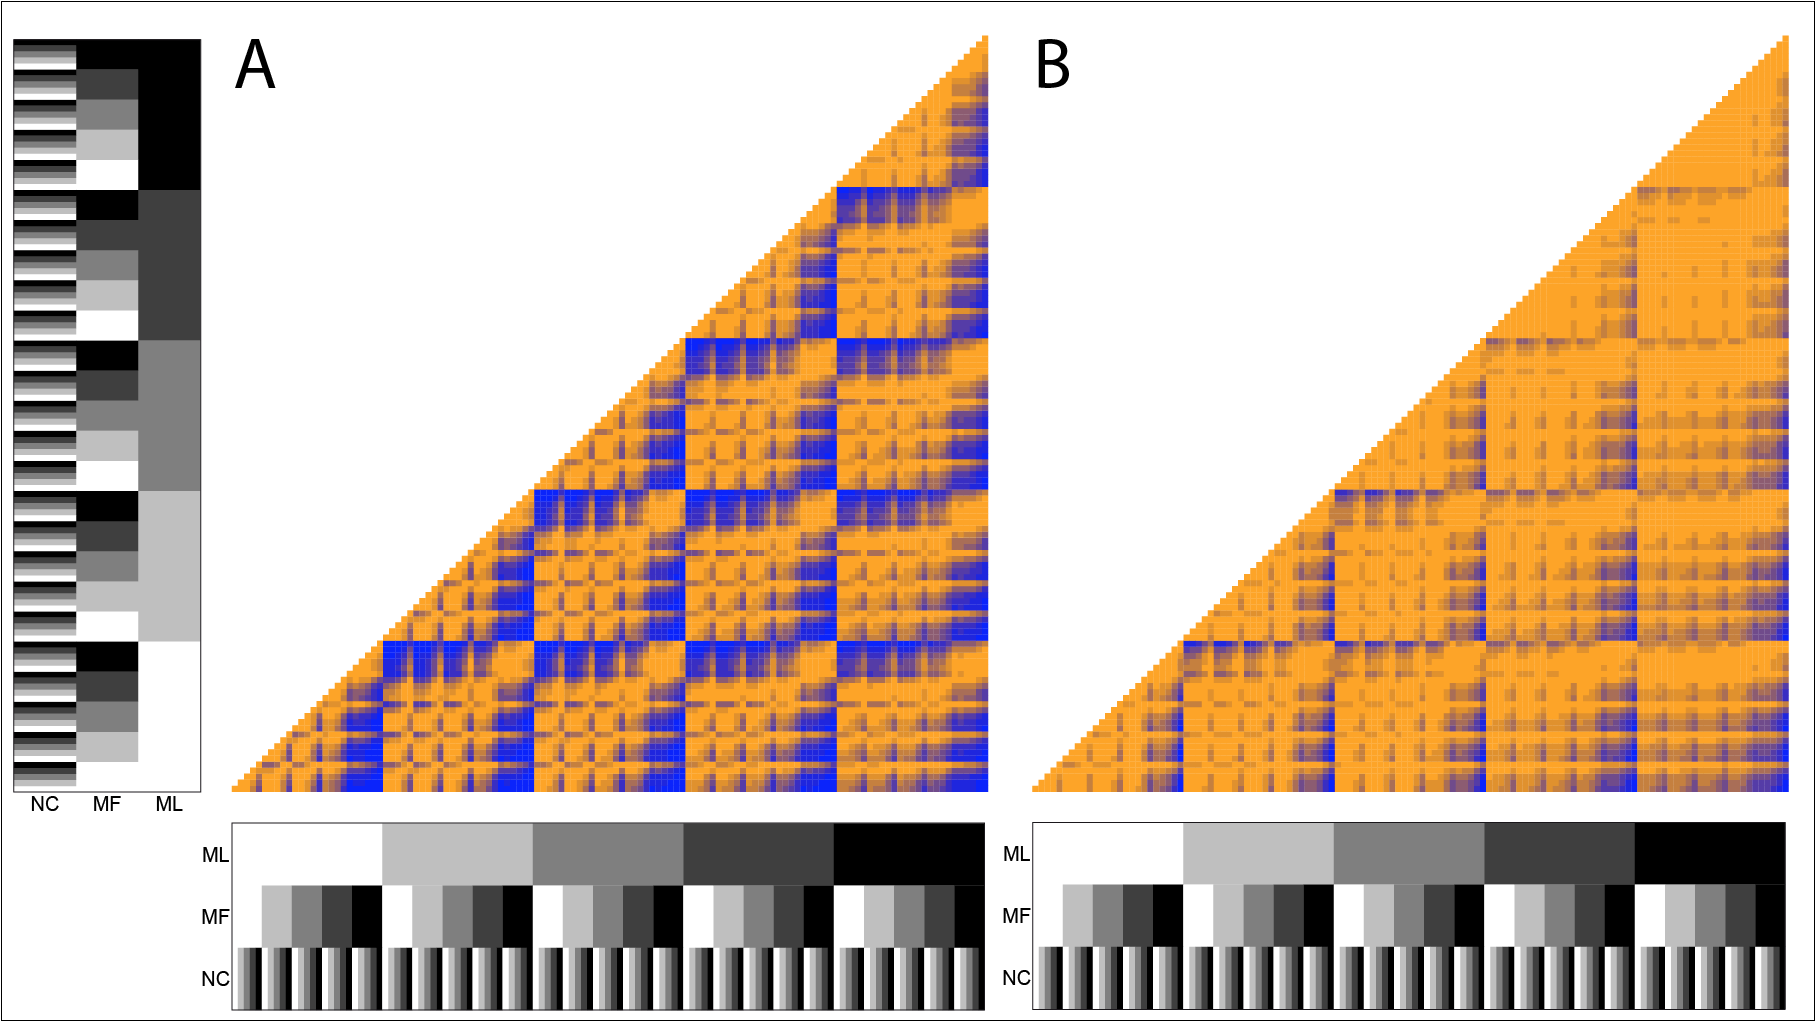
\includegraphics[width=1\textwidth]{Figures/Supplementary/PairwiseComp-Boot-RF+Tr-colour.pdf}
    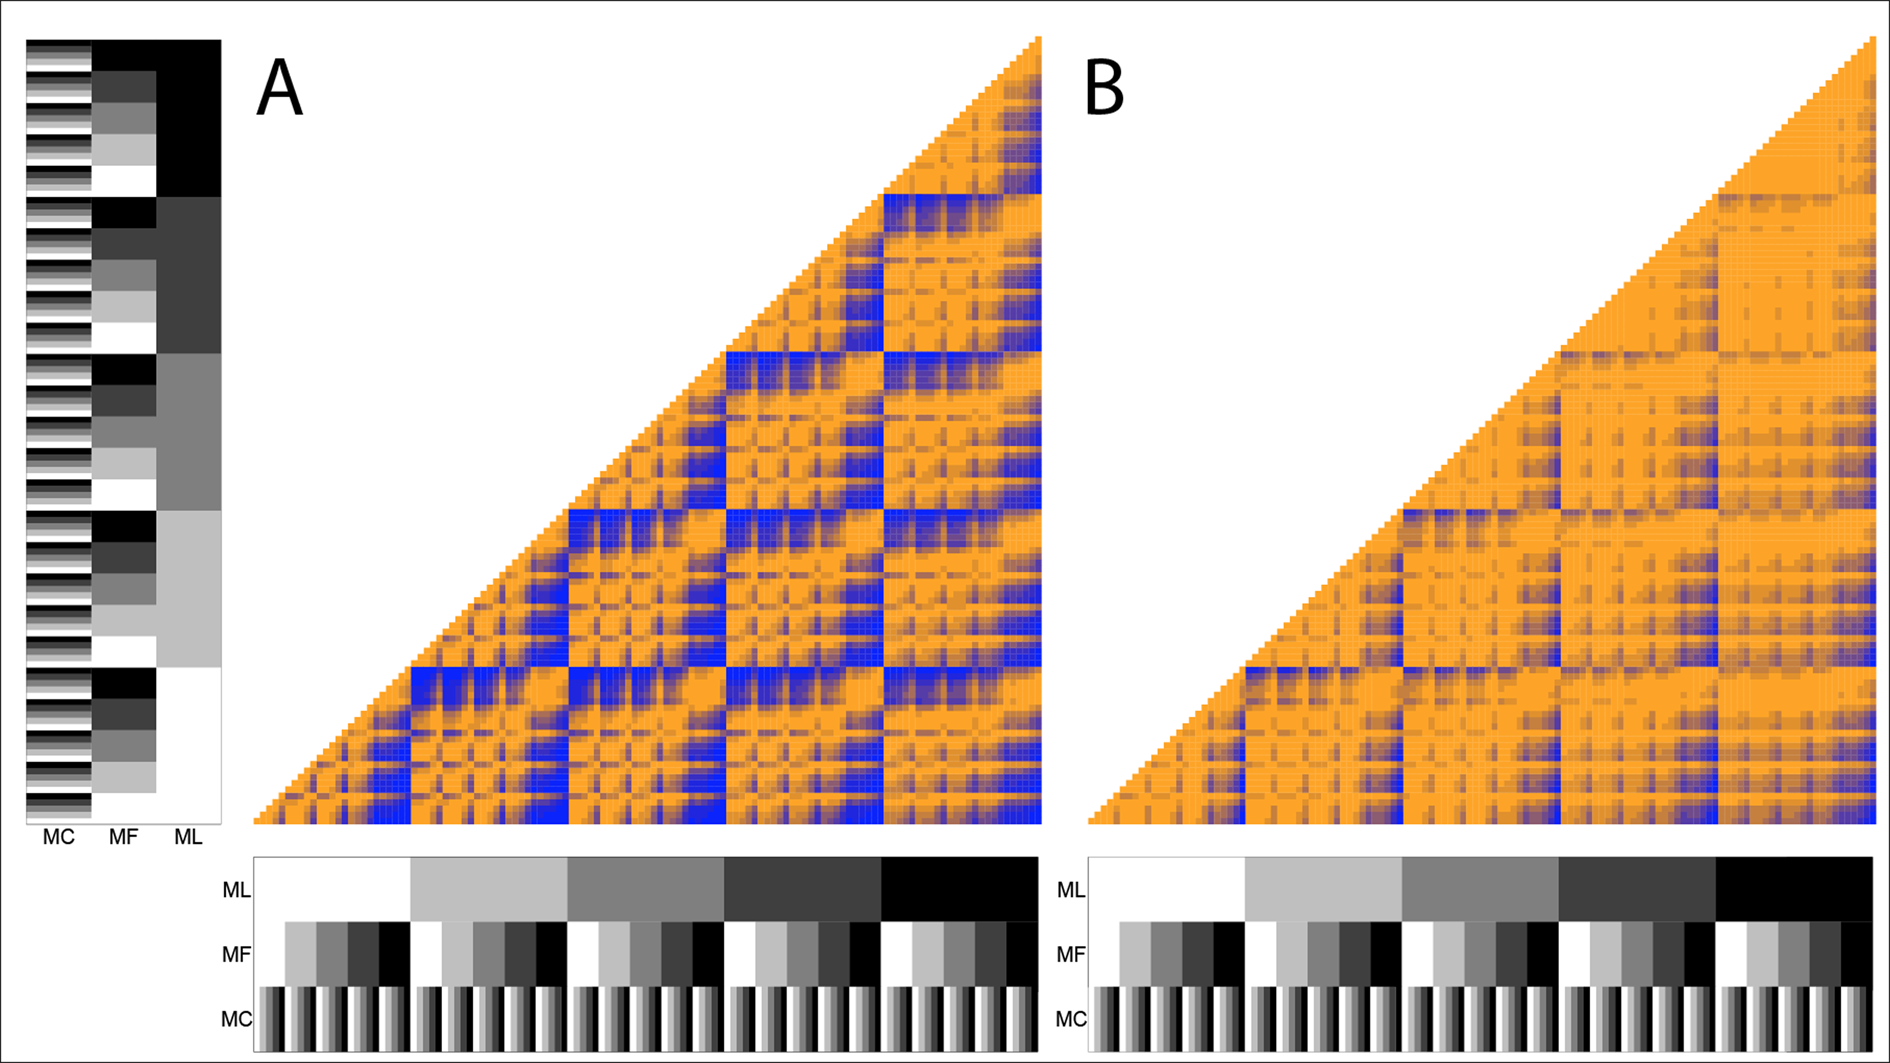
\includegraphics[width=1\textwidth]{OnlineAppendices-LaTeXSuppFiles/SupplementaryFigures/PairwiseComp-Boot-RF+Tr-colour.png} %bitmap version - 300 dpi RGB
    \caption{The effects of missing data on topological recovery using Maximum Likelihood bootstrap trees. The x and the y axes both show show the percentage of missing data from 0\% (white) to 75\% (black) for the three parameters: $M_{L}$ (upper line), $M_{F}$ (middle line) and $M_{C}$ (lower line). Topological recovery is represented by the probability of (A) Normalised Robinson-Foulds distance and (B) Normalised Triplets distance distributions overlapping with the "best" tree distribution, calculated using the Bhattacharyya Coefficient. The Bhattacharyya Coefficient values are indicated using a color gradient ranging from low probability of overlap in blue, to a high probability of overlap in orange.}
\label{Fig_Supp_paircomp_Boot}
\end{figure} 

\begin{figure} 
\centering
     %Hide this figure for 'fast' build
%    \includegraphics[width=1\textwidth]{Figures/Supplementary/PPairwiseComp-Bayt-RF+Tr-colour.pdf}
    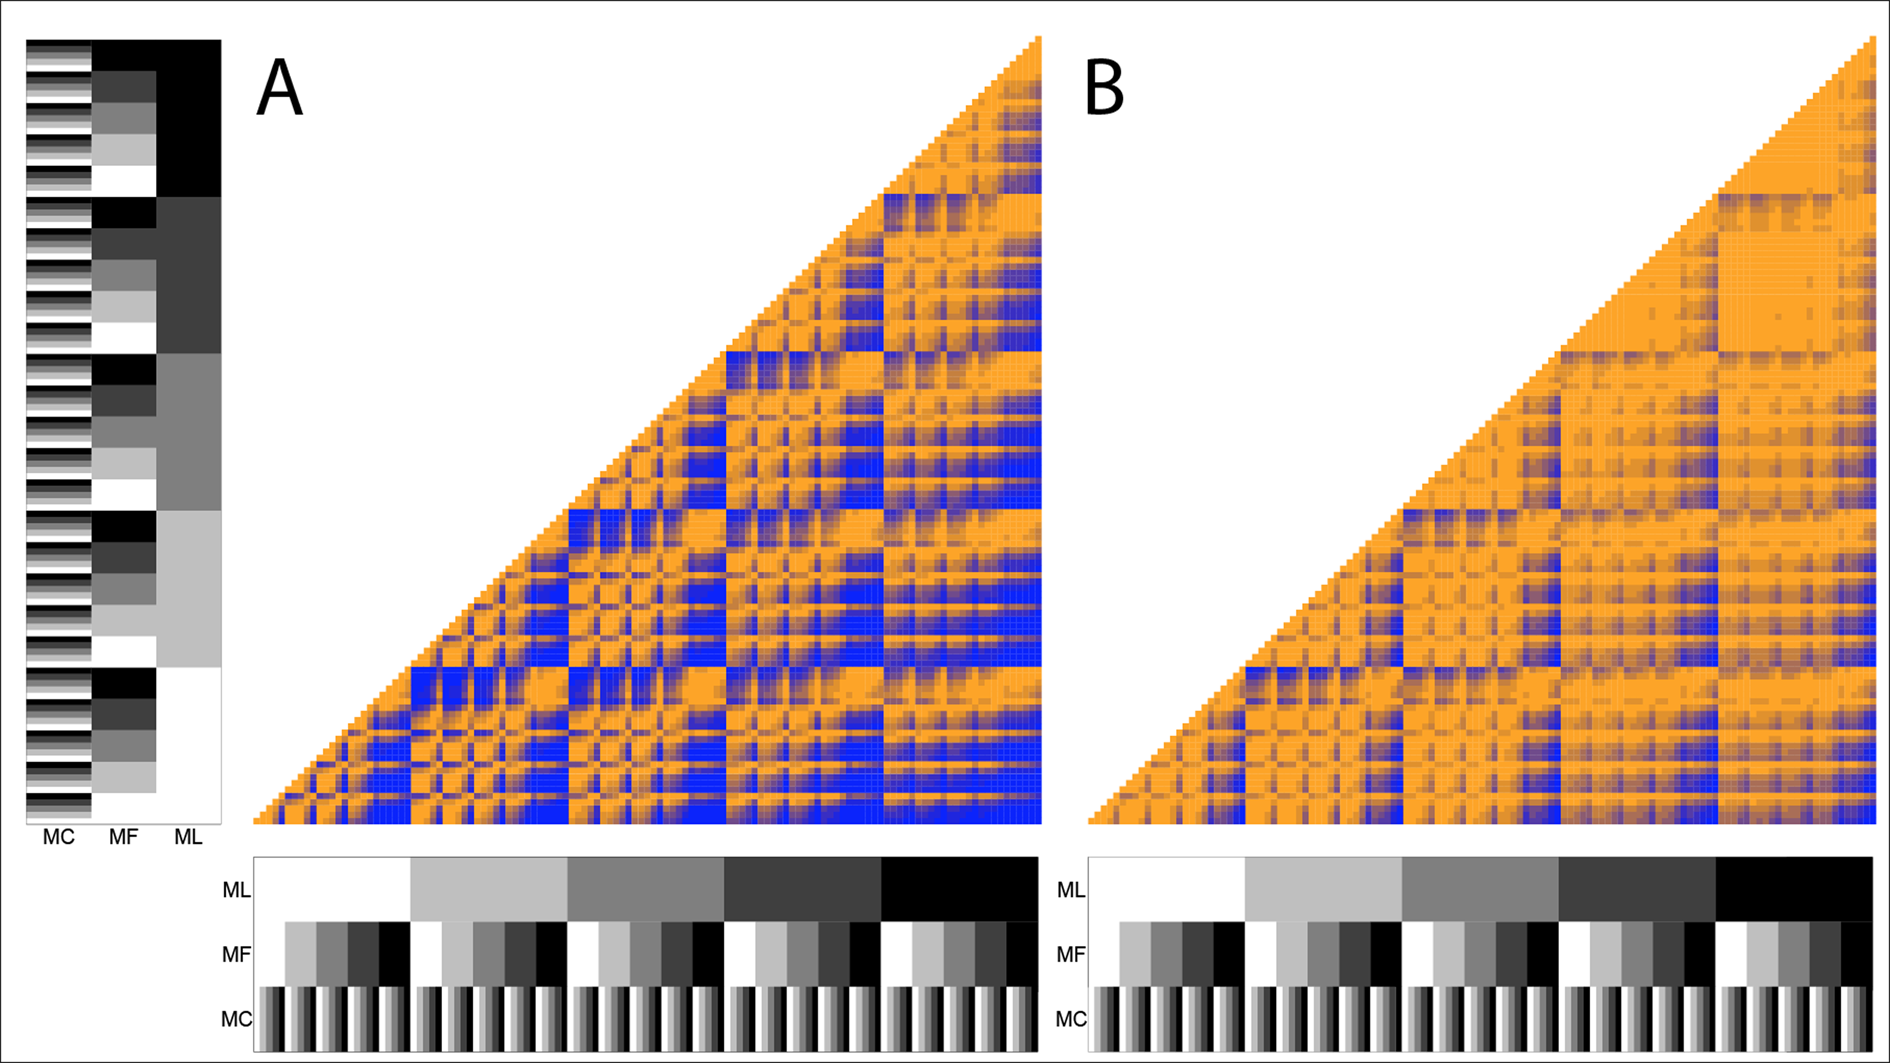
\includegraphics[width=1\textwidth]{OnlineAppendices-LaTeXSuppFiles/SupplementaryFigures/PairwiseComp-Bayt-RF+Tr-colour.png} %bitmap version - 300 dpi RGB
    \caption{The effects of missing data on topological recovery using Bayesian posterior tree distribution. The x and the y axes both show show the percentage of missing data from 0\% (white) to 75\% (black) for the three parameters: $M_{L}$ (upper line), $M_{F}$ (middle line) and $M_{C}$ (lower line). Topological recovery is represented by the probability of (A) Normalised Robinson-Foulds distance and (B) Normalised Triplets distance distributions overlapping with the "best" tree distribution, calculated using the Bhattacharyya Coefficient. TThe Bhattacharyya Coefficient values are indicated using a color gradient ranging from low probability of overlap in blue, to a high probability of overlap in orange.}
\label{Fig_Supp_paircomp_Bayt}
\end{figure} 


%Summary of metrics values for all parameters combinations
\begin{landscape}
\begin{table}[ht]
\caption{Summary of the of the comparisons between the "best" tree and the "missing data" trees for each different tree inference method using either the Normalised Robinson-Foulds distance (RF) or the Normalised Triplets distance (Tr).}
\label{Tab_Supp_summary_metric_allparam}
\centering
\begin{tabular}{lccccccc}
  \hline
 Tree inference method & Metric & Min. & 1st Qu. & Median & Mean & 3rd Qu. & Max. \\ 
  \hline
  Maximum Likelihood                    & $RF$ & 0.06 & 0.26 & 0.40 & 0.41 & 0.50 & 0.95 \\ 
                                        & $Tr$ & 0.29 & 0.45 & 0.59 & 0.63 & 0.84 & 1.00 \\ 
  Bayesian consensus                    & $RF$ & 0.69 & 0.71 & 0.72 & 0.76 & 0.79 & 0.96 \\ 
                                        & $Tr$ & -0.28 & -0.11 & 0.17 & 0.19 & 0.37 & 0.98 \\ 
  Maximum Likelihood bootstraps         & $RF$ & 0.06 & 0.18 & 0.27 & 0.26 & 0.34 & 0.46 \\ 
                                        & $Tr$ & 0.23 & 0.31 & 0.35 & 0.38 & 0.45 & 0.58 \\ 
  Bayesian posterior tree distributions & $RF$ & 0.16 & 0.22 & 0.32 & 0.34 & 0.42 & 0.65 \\ 
                                        & $Tr$ & 0.24 & 0.35 & 0.40 & 0.50 & 0.67 & 0.98 \\ 
   \hline
\end{tabular}
\end{table}
\end{landscape}


%Summary of metrics values for the ML parameter
\begin{landscape}
\begin{table}[ht]
\caption{Summary of the of the comparisons between the "best" tree and the "missing data" trees for each different tree inference method using either the Normalised Robinson-Foulds distance (RF) or the Normalised Triplets distance (Tr) for the $M_{L}$ missing data parameter only.}
\label{Tab_Supp_summary_metric_ML}
\centering
\begin{tabular}{lccccccc}
  \hline
 Tree inference method & Metric & Min. & 1st Qu. & Median & Mean & 3rd Qu. & Max. \\ 
  \hline
  Maximum Likelihood                    & $RF$ & 0.44 & 0.51 & 0.63 & 0.66 & 0.78 & 0.95 \\ 
                                        & $Tr$ & 0.45 & 0.56 & 0.76 & 0.74 & 0.93 & 0.99 \\ 
  Bayesian consensus                    & $RF$ & 0.71 & 0.73 & 0.80 & 0.82 & 0.88 & 0.95 \\ 
                                        & $Tr$ & 0.37 & 0.46 & 0.67 & 0.67 & 0.87 & 0.96 \\ 
  Maximum Likelihood bootstraps         & $RF$ & 0.34 & 0.37 & 0.42 & 0.41 & 0.44 & 0.46 \\ 
                                        & $Tr$ & 0.32 & 0.40 & 0.51 & 0.46 & 0.51 & 0.57 \\ 
  Bayesian posterior tree distributions & $RF$ & 0.33 & 0.41 & 0.52 & 0.50 & 0.60 & 0.65 \\ 
                                        & $Tr$ & 0.41 & 0.56 & 0.76 & 0.71 & 0.84 & 0.98 \\ 
   \hline
\end{tabular}
\end{table}
\end{landscape}


%Summary of metrics values for the MF parameter
\begin{landscape}
\begin{table}[ht]
\caption{Summary of the of the comparisons between the "best" tree and the "missing data" trees for each different tree inference method using either the Normalised Robinson-Foulds distance (RF) or the Normalised Triplets distance (Tr) for the $M_{F}$ missing data parameter only.}
\label{Tab_Supp_summary_metric_MF}
\centering
\begin{tabular}{lccccccc}
  \hline
 Tree inference method & Metric & Min. & 1st Qu. & Median & Mean & 3rd Qu. & Max. \\ 
  \hline
  Maximum Likelihood                    & $RF$ & 0.23 & 0.46 & 0.64 & 0.61 & 0.79 & 0.93 \\ 
                                        & $Tr$ & 0.65 & 0.84 & 0.95 & 0.89 & 0.99 & 1.00 \\ 
  Bayesian consensus                    & $RF$ & 0.72 & 0.77 & 0.86 & 0.85 & 0.94 & 0.96 \\ 
                                        & $Tr$ & -0.16 & 0.19 & 0.63 & 0.52 & 0.96 & 0.98 \\ 
  Maximum Likelihood bootstraps         & $RF$ & 0.14 & 0.30 & 0.40 & 0.35 & 0.45 & 0.46 \\ 
                                        & $Tr$ & 0.37 & 0.49 & 0.54 & 0.51 & 0.56 & 0.57 \\ 
  Bayesian posterior tree distributions & $RF$ & 0.24 & 0.45 & 0.57 & 0.51 & 0.63 & 0.65 \\ 
                                        & $Tr$ & 0.44 & 0.81 & 0.86 & 0.82 & 0.98 & 0.98 \\ 
   \hline
\end{tabular}
\end{table}
\end{landscape}

%Summary of metrics values for the MC parameter
\begin{landscape}
\begin{table}[ht]
\caption{Summary of the of the comparisons between the "best" tree and the "missing data" trees for each different tree inference method using either the Normalised Robinson-Foulds distance (RF) or the Normalised Triplets distance (Tr) for the $M_{C}$ missing data parameter only.}
\label{Tab_Supp_summary_metric_MC}
\centering
\begin{tabular}{lccccccc}
  \hline
 Tree inference method & Metric & Min. & 1st Qu. & Median & Mean & 3rd Qu. & Max. \\ 
  \hline
  Maximum Likelihood                    & $RF$ & 0.40 & 0.50 & 0.64 & 0.65 & 0.79 & 0.94 \\ 
                                        & $Tr$ & 0.70 & 0.84 & 0.93 & 0.89 & 0.99 & 1.00 \\ 
  Bayesian consensus                    & $RF$ & 0.76 & 0.79 & 0.86 & 0.86 & 0.92 & 0.96 \\ 
                                        & $Tr$ & 0.05 & 0.16 & 0.53 & 0.50 & 0.87 & 0.92 \\ 
  Maximum Likelihood bootstraps         & $RF$ & 0.25 & 0.34 & 0.42 & 0.38 & 0.45 & 0.46 \\ 
                                        & $Tr$ & 0.38 & 0.47 & 0.55 & 0.51 & 0.57 & 0.58 \\ 
  Bayesian posterior tree distributions & $RF$ & 0.32 & 0.44 & 0.58 & 0.52 & 0.62 & 0.65 \\ 
                                        & $Tr$ & 0.39 & 0.78 & 0.82 & 0.79 & 0.98 & 0.98 \\ 
   \hline
\end{tabular}
\end{table}
\end{landscape}


%Summary of the BC between pairs of methods for the ML parameter
\begin{landscape}
\begin{table}[ht]
\caption{Bhattacharyya Coefficients of the pairwise method comparisons, each of which corresponds to the normalised distance between the "best" tree and the "missing data" using either the Normalised Robinson-Foulds distance (RF) or the Normalised Triplets distance (Tr) for the $M_{L}$ missing data parameter only.}
\label{Tab_Supp_summary_BC_ML}
\centering
\begin{tabular}{lccccccc}
  \hline
 Comparison &  Metric & Min. & 1st Qu. & Median & Mean & 3rd Qu. & Max. \\ 
  \hline
    Maximum Likelihood \textit{vs.} Bayesian consensus                 & $RF$ & 0.30 & 0.31 & 0.69 & 0.61 & 0.77 & 1.00 \\ 
                                                                       & $Tr$ & 0.79 & 0.81 & 0.84 & 0.86 & 0.85 & 1.00 \\ 
    Maximum Likelihood \textit{vs.} Maximum Likelihood bootstraps      & $RF$ & 0.03 & 0.22 & 0.29 & 0.36 & 0.54 & 0.69 \\ 
                                                                       & $Tr$ & 0.08 & 0.42 & 0.53 & 0.51 & 0.74 & 0.78 \\ 
    Maximum Likelihood \textit{vs.} Bayesian posterior trees           & $RF$ & 0.02 & 0.49 & 0.61 & 0.51 & 0.67 & 0.74 \\ 
                                                                       & $Tr$ & 0.21 & 0.61 & 0.70 & 0.63 & 0.81 & 0.81 \\ 
    Bayesian consensus \textit{vs.} Maximum Likelihood bootstraps      & $RF$ & 0.01 & 0.02 & 0.02 & 0.02 & 0.03 & 0.04 \\ 
                                                                       & $Tr$ & 0.08 & 0.69 & 0.78 & 0.64 & 0.79 & 0.84 \\ 
    Bayesian consensus \textit{vs.} Bayesian posterior trees           & $RF$ & 0.01 & 0.02 & 0.02 & 0.04 & 0.08 & 0.09 \\ 
                                                                       & $Tr$ & 0.21 & 0.74 & 0.75 & 0.68 & 0.84 & 0.87 \\ 
    Bayesian posterior tree \textit{vs.} Maximum Likelihood bootstraps & $RF$ & 0.69 & 0.75 & 0.85 & 0.85 & 0.95 & 1.00 \\ 
                                                                       & $Tr$ & 0.91 & 0.92 & 0.96 & 0.95 & 0.97 & 0.98 \\ 
   \hline
\end{tabular}
\end{table}
\end{landscape}

%Summary of the BC between pairs of methods for the MF parameter
\begin{landscape}
\begin{table}[ht]
\caption{Bhattacharyya Coefficients of the pairwise method comparisons, each of which corresponds to the normalised distance between the "best" tree and the "missing data" using either the Normalised Robinson-Foulds distance (RF) or the Normalised Triplets distance (Tr) for the $M_{F}$ missing data parameter only.}
\label{Tab_Supp_summary_BC_MF}
\centering
\begin{tabular}{lccccccc}
  \hline
 Comparison &  Metric & Min. & 1st Qu. & Median & Mean & 3rd Qu. & Max. \\  
  \hline
    Maximum Likelihood \textit{vs.} Bayesian consensus                 & $RF$ & 0.00 & 0.25 & 0.48 & 0.50 & 0.76 & 1.00 \\ 
                                                                       & $Tr$ & 0.38 & 0.69 & 0.75 & 0.72 & 0.80 & 1.00 \\ 
    Maximum Likelihood \textit{vs.} Maximum Likelihood bootstraps      & $RF$ & 0.03 & 0.18 & 0.32 & 0.36 & 0.47 & 0.77 \\ 
                                                                       & $Tr$ & 0.08 & 0.34 & 0.40 & 0.38 & 0.53 & 0.55 \\ 
    Maximum Likelihood \textit{vs.} Bayesian posterior trees           & $RF$ & 0.02 & 0.47 & 0.71 & 0.60 & 0.86 & 0.94 \\ 
                                                                       & $Tr$ & 0.21 & 0.54 & 0.62 & 0.56 & 0.64 & 0.80 \\ 
    Bayesian consensus \textit{vs.} Maximum Likelihood bootstraps      & $RF$ & 0.00 & 0.00 & 0.01 & 0.01 & 0.01 & 0.03 \\ 
                                                                       & $Tr$ & 0.08 & 0.38 & 0.54 & 0.49 & 0.70 & 0.75 \\ 
    Bayesian consensus \textit{vs.} Bayesian posterior trees           & $RF$ & 0.00 & 0.02 & 0.02 & 0.02 & 0.04 & 0.04 \\ 
                                                                       & $Tr$ & 0.21 & 0.29 & 0.66 & 0.54 & 0.72 & 0.82 \\ 
    Bayesian posterior tree \textit{vs.} Maximum Likelihood bootstraps & $RF$ & 0.69 & 0.69 & 0.72 & 0.71 & 0.72 & 0.72 \\ 
                                                                       & $Tr$ & 0.91 & 0.91 & 0.91 & 0.93 & 0.92 & 0.98 \\ 
   \hline
\end{tabular}
\end{table}
\end{landscape}

%Summary of the BC between pairs of methods for the MC parameter
\begin{landscape}
\begin{table}[ht]
\caption{Bhattacharyya Coefficients of the pairwise method comparisons, each of which corresponds to the normalised distance between the "best" tree and the "missing data" using either the Normalised Robinson-Foulds distance (RF) or the Normalised Triplets distance (Tr) for the $M_{C}$ missing data parameter only.}
\label{Tab_Supp_summary_BC_MC}
\centering
\begin{tabular}{lccccccc}
  \hline
 Comparison &  Metric & Min. & 1st Qu. & Median & Mean & 3rd Qu. & Max. \\  
  \hline
    Maximum Likelihood \textit{vs.} Bayesian consensus                 & $RF$ & 0.03 & 0.32 & 0.66 & 0.55 & 0.75 & 1.00 \\ 
                                                                       & $Tr$ & 0.51 & 0.69 & 0.80 & 0.76 & 0.80 & 1.00 \\ 
    Maximum Likelihood \textit{vs.} Maximum Likelihood bootstraps      & $RF$ & 0.03 & 0.17 & 0.21 & 0.31 & 0.46 & 0.68 \\ 
                                                                       & $Tr$ & 0.08 & 0.31 & 0.39 & 0.39 & 0.56 & 0.61 \\ 
    Maximum Likelihood \textit{vs.} Bayesian posterior trees           & $RF$ & 0.02 & 0.44 & 0.47 & 0.52 & 0.78 & 0.90 \\ 
                                                                       & $Tr$ & 0.21 & 0.52 & 0.59 & 0.55 & 0.66 & 0.77 \\ 
    Bayesian consensus \textit{vs.} Maximum Likelihood bootstraps      & $RF$ & 0.00 & 0.01 & 0.01 & 0.02 & 0.02 & 0.03 \\ 
                                                                       & $Tr$ & 0.08 & 0.47 & 0.62 & 0.51 & 0.66 & 0.73 \\ 
    Bayesian consensus \textit{vs.} Bayesian posterior trees           & $RF$ & 0.00 & 0.02 & 0.04 & 0.04 & 0.05 & 0.06 \\ 
                                                                       & $Tr$ & 0.21 & 0.45 & 0.64 & 0.57 & 0.74 & 0.79 \\ 
    Bayesian posterior tree \textit{vs.} Maximum Likelihood bootstraps & $RF$ & 0.69 & 0.73 & 0.73 & 0.76 & 0.81 & 0.86 \\ 
                                                                       & $Tr$ & 0.91 & 0.92 & 0.93 & 0.94 & 0.96 & 0.99 \\ 
   \hline
\end{tabular}
\end{table}
\end{landscape}